\section{Results }
\label{sec:results}

\subsection{Differential Model and Simple Agent-Based Model}
\label{subsec:basicmod}

\begin{figure}[H]
\captionsetup{width=0.6\textwidth}
\centering
    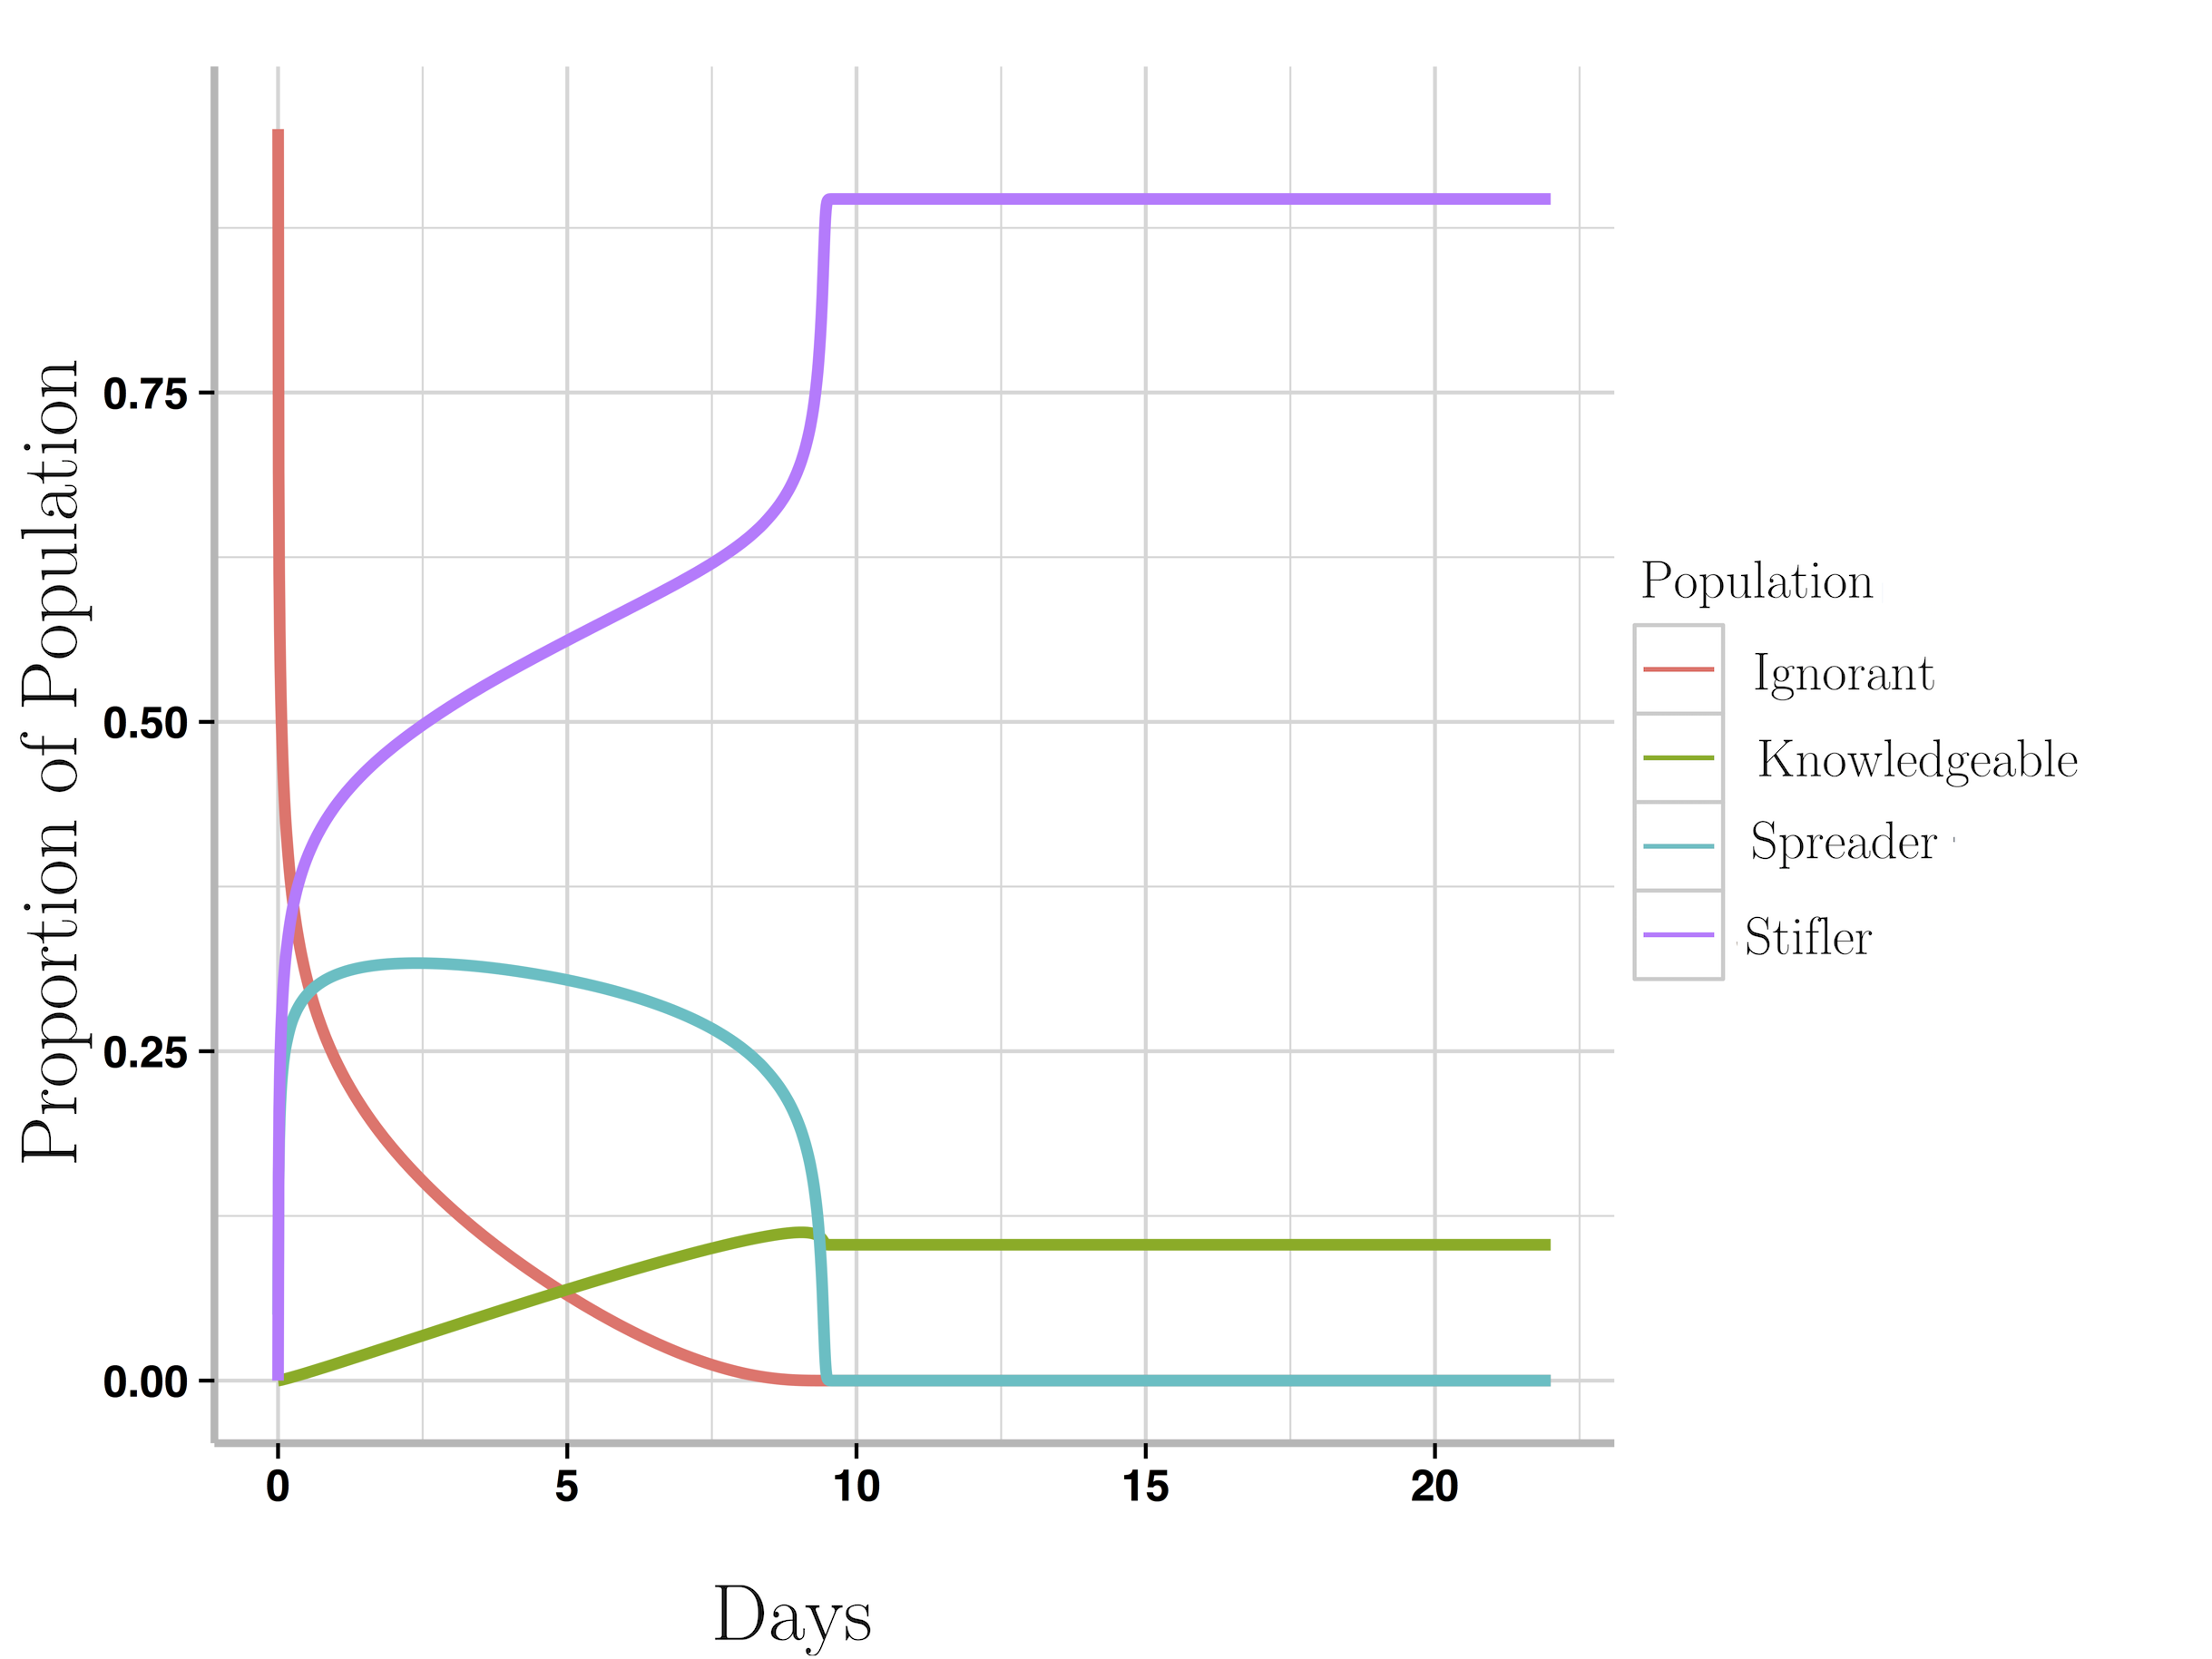
\includegraphics[width=0.7\textwidth]{figures/figure1}
  \caption{ Differential model proportions of the population in each class over 22 days.}
\label{fig:figure1}
\end{figure}

For the differential model, as is demonstrated in Figure~\ref{fig:figure1}, the spreader and ignorant populations become negligible by the end of the 22 days, and the knowledgeable and stifler populations stabilize above 0.
The ignorant population declines, as the spreader population initially grows, and then declines as the stifler population grows.
In the differential model, essentially all individuals learn about the rumor.
Varying the parameters impacts how quickly the population hears of the rumor, but not the ignorant and spreader populations.

\begin{figure}[H]
\captionsetup{width=0.8\textwidth}
\centering
    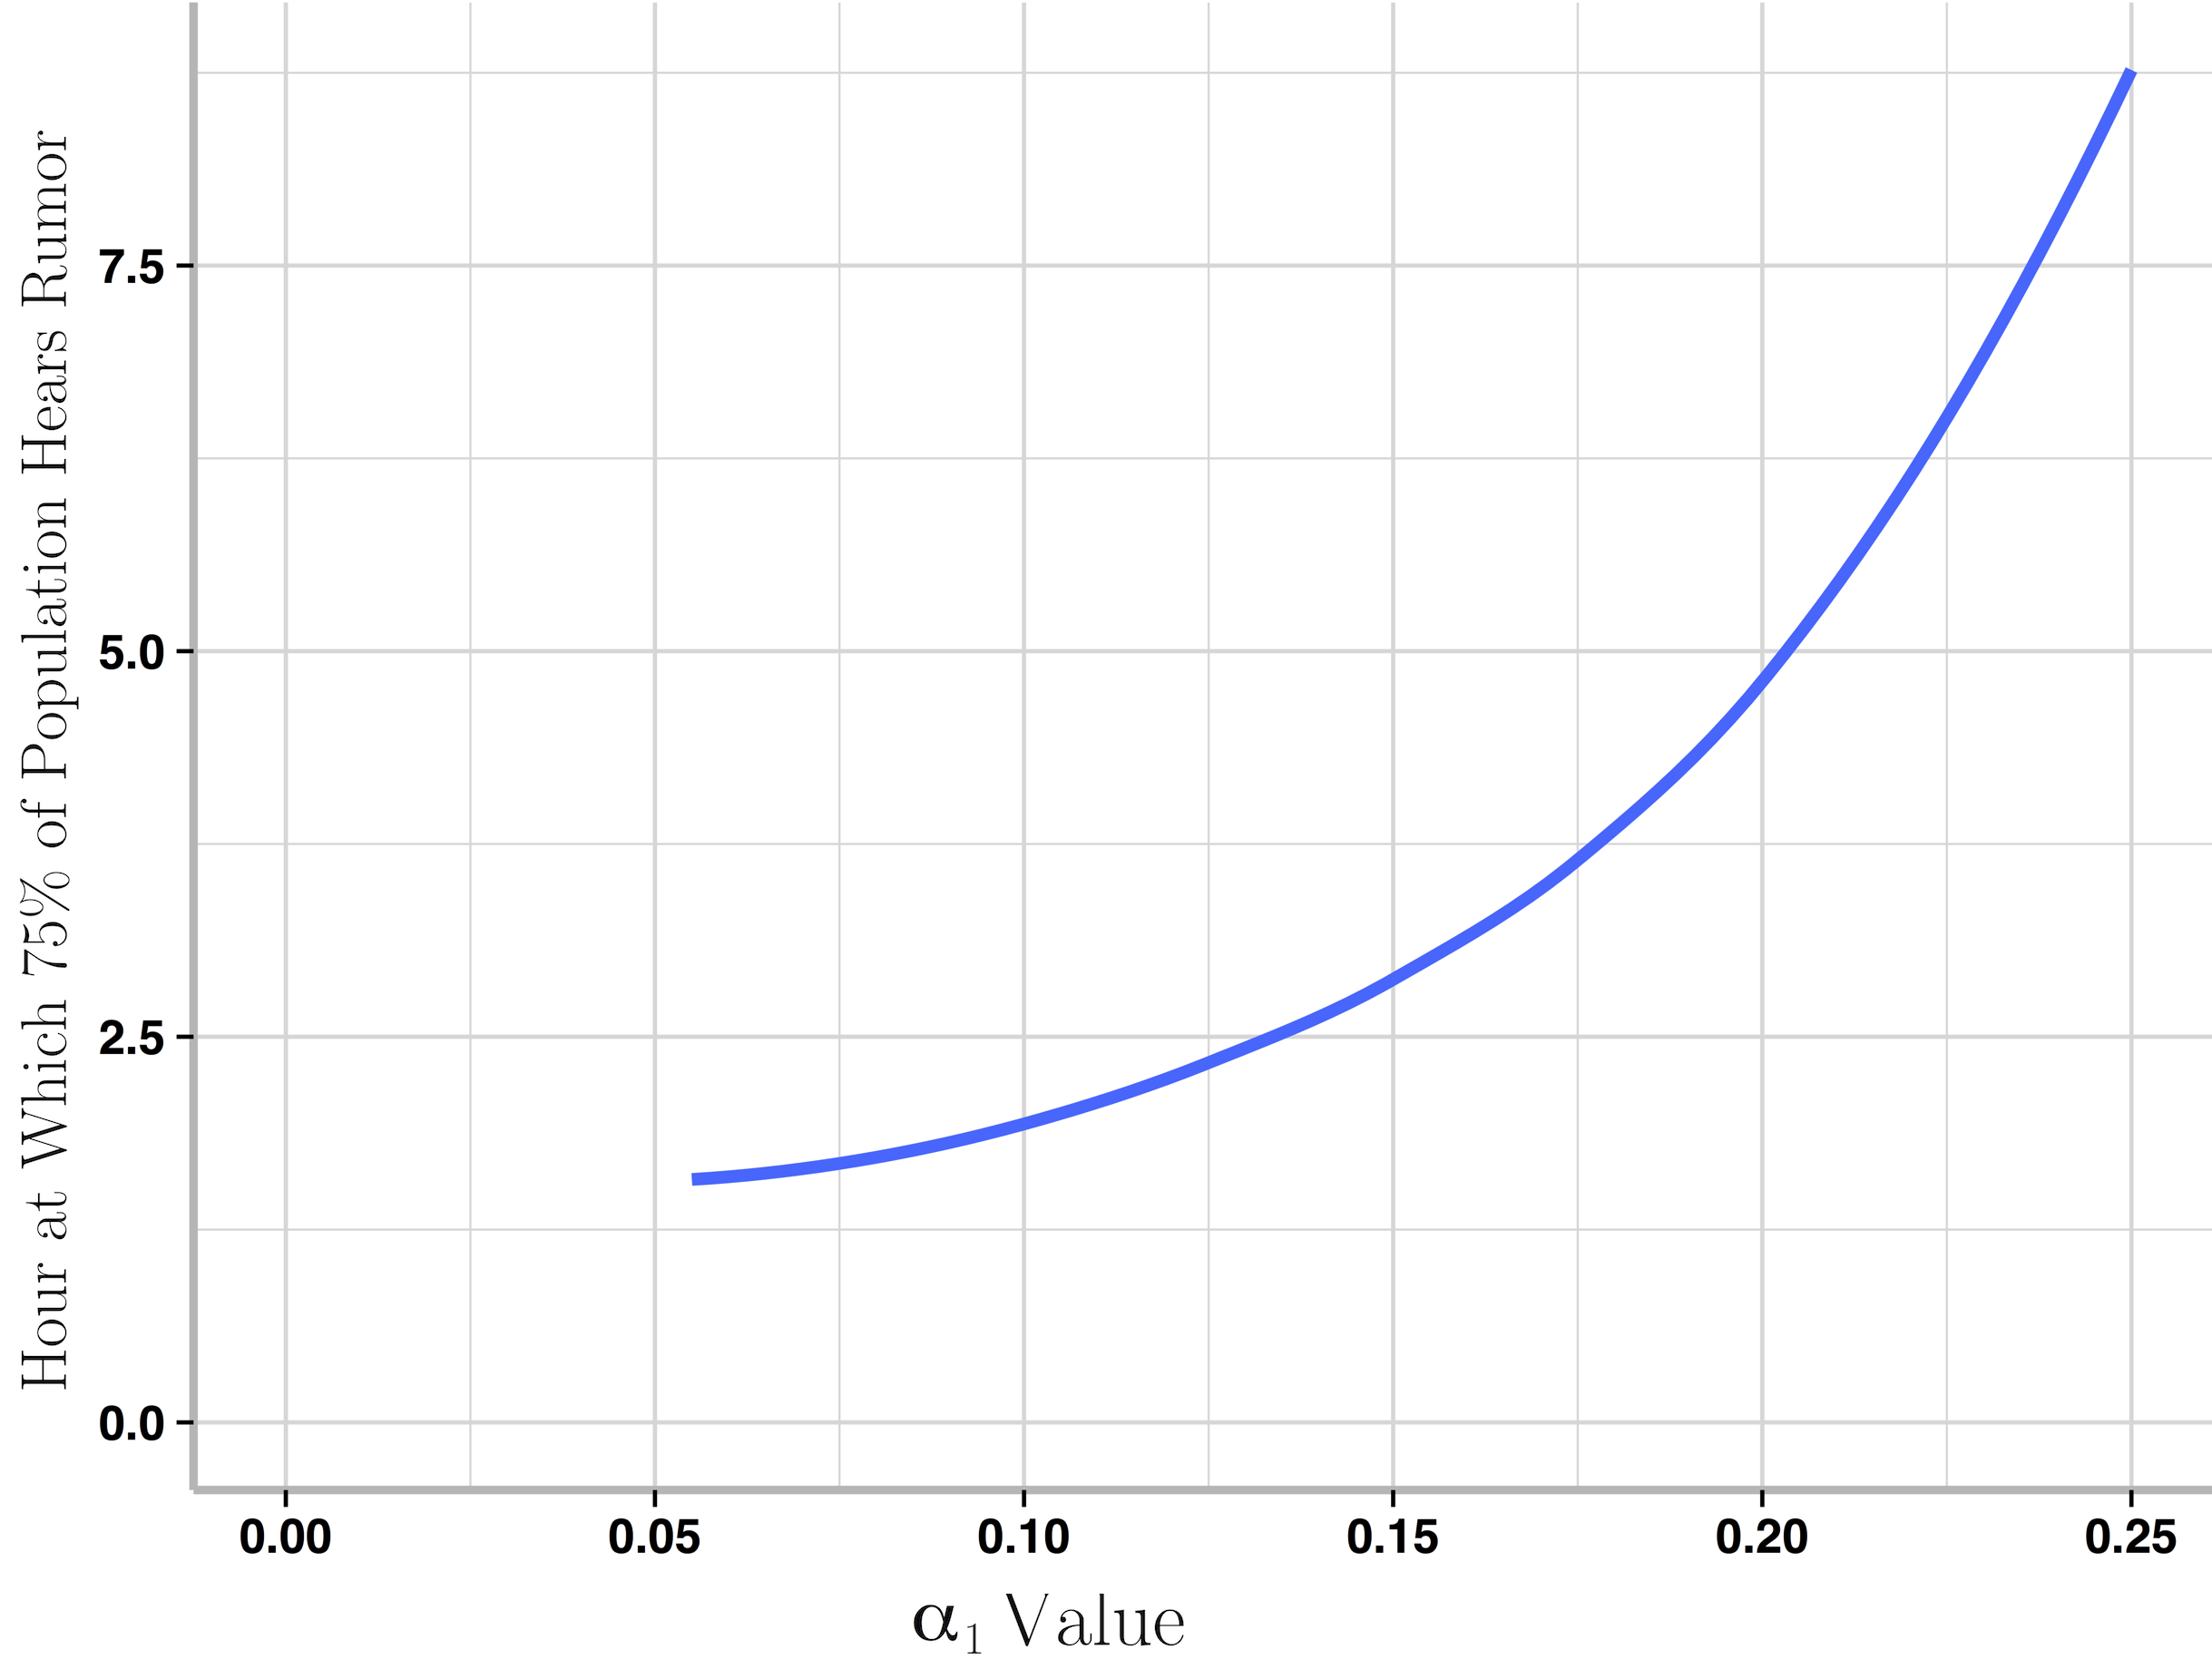
\includegraphics[width=0.7\textwidth]{figures/figure2}
  \caption{ Results of the sensitivity analysis of parameter $ \alpha_1 $ in the differential model.
For each value of $ \alpha_1 $ the time at which 75\% of the population had been exposed to the rumor is recorded.}
\label{fig:figure2}
\end{figure}

\begin{figure}[H]
\captionsetup{width=0.8\textwidth}
\centering
    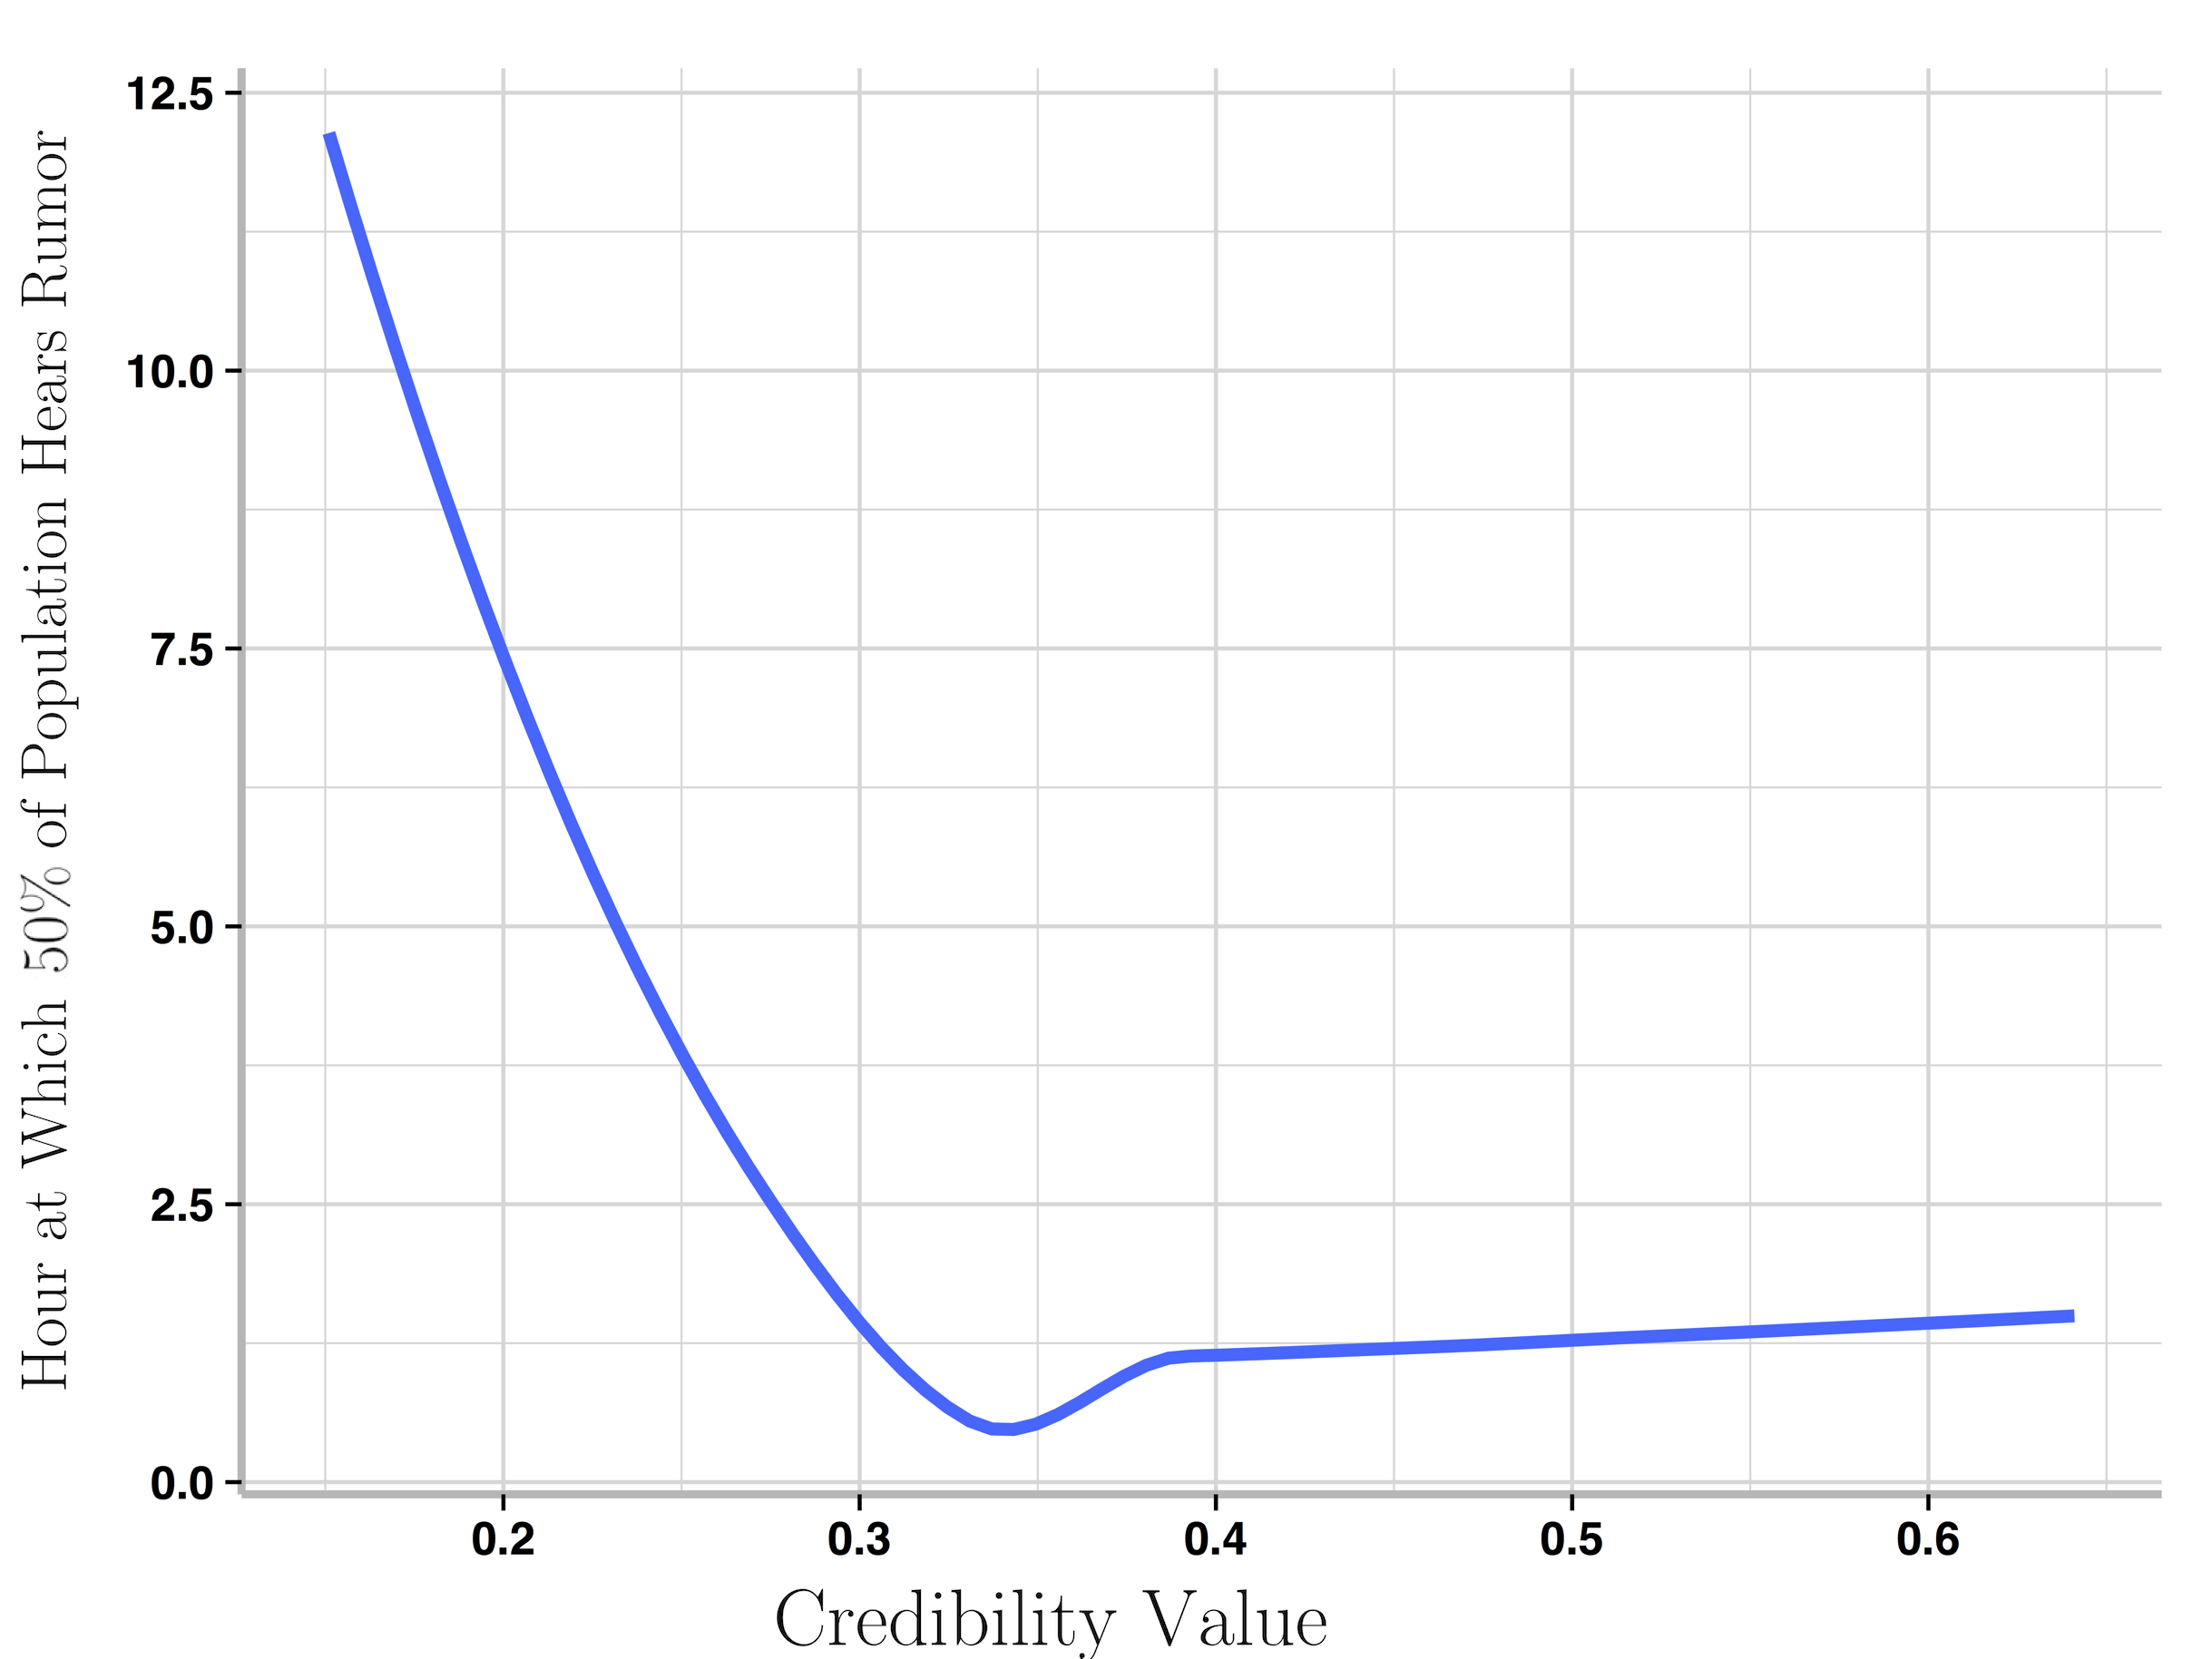
\includegraphics[width=0.7\textwidth]{figures/figure3}
  \caption{ Sensitivity analysis of parameter $ c $ in the differential model.
For each credibility value the time at which 50\% of the population heard the rumor }
\label{fig:figure3}
\end{figure}

\begin{figure}[H]
\captionsetup{width=0.8\textwidth}
\centering
    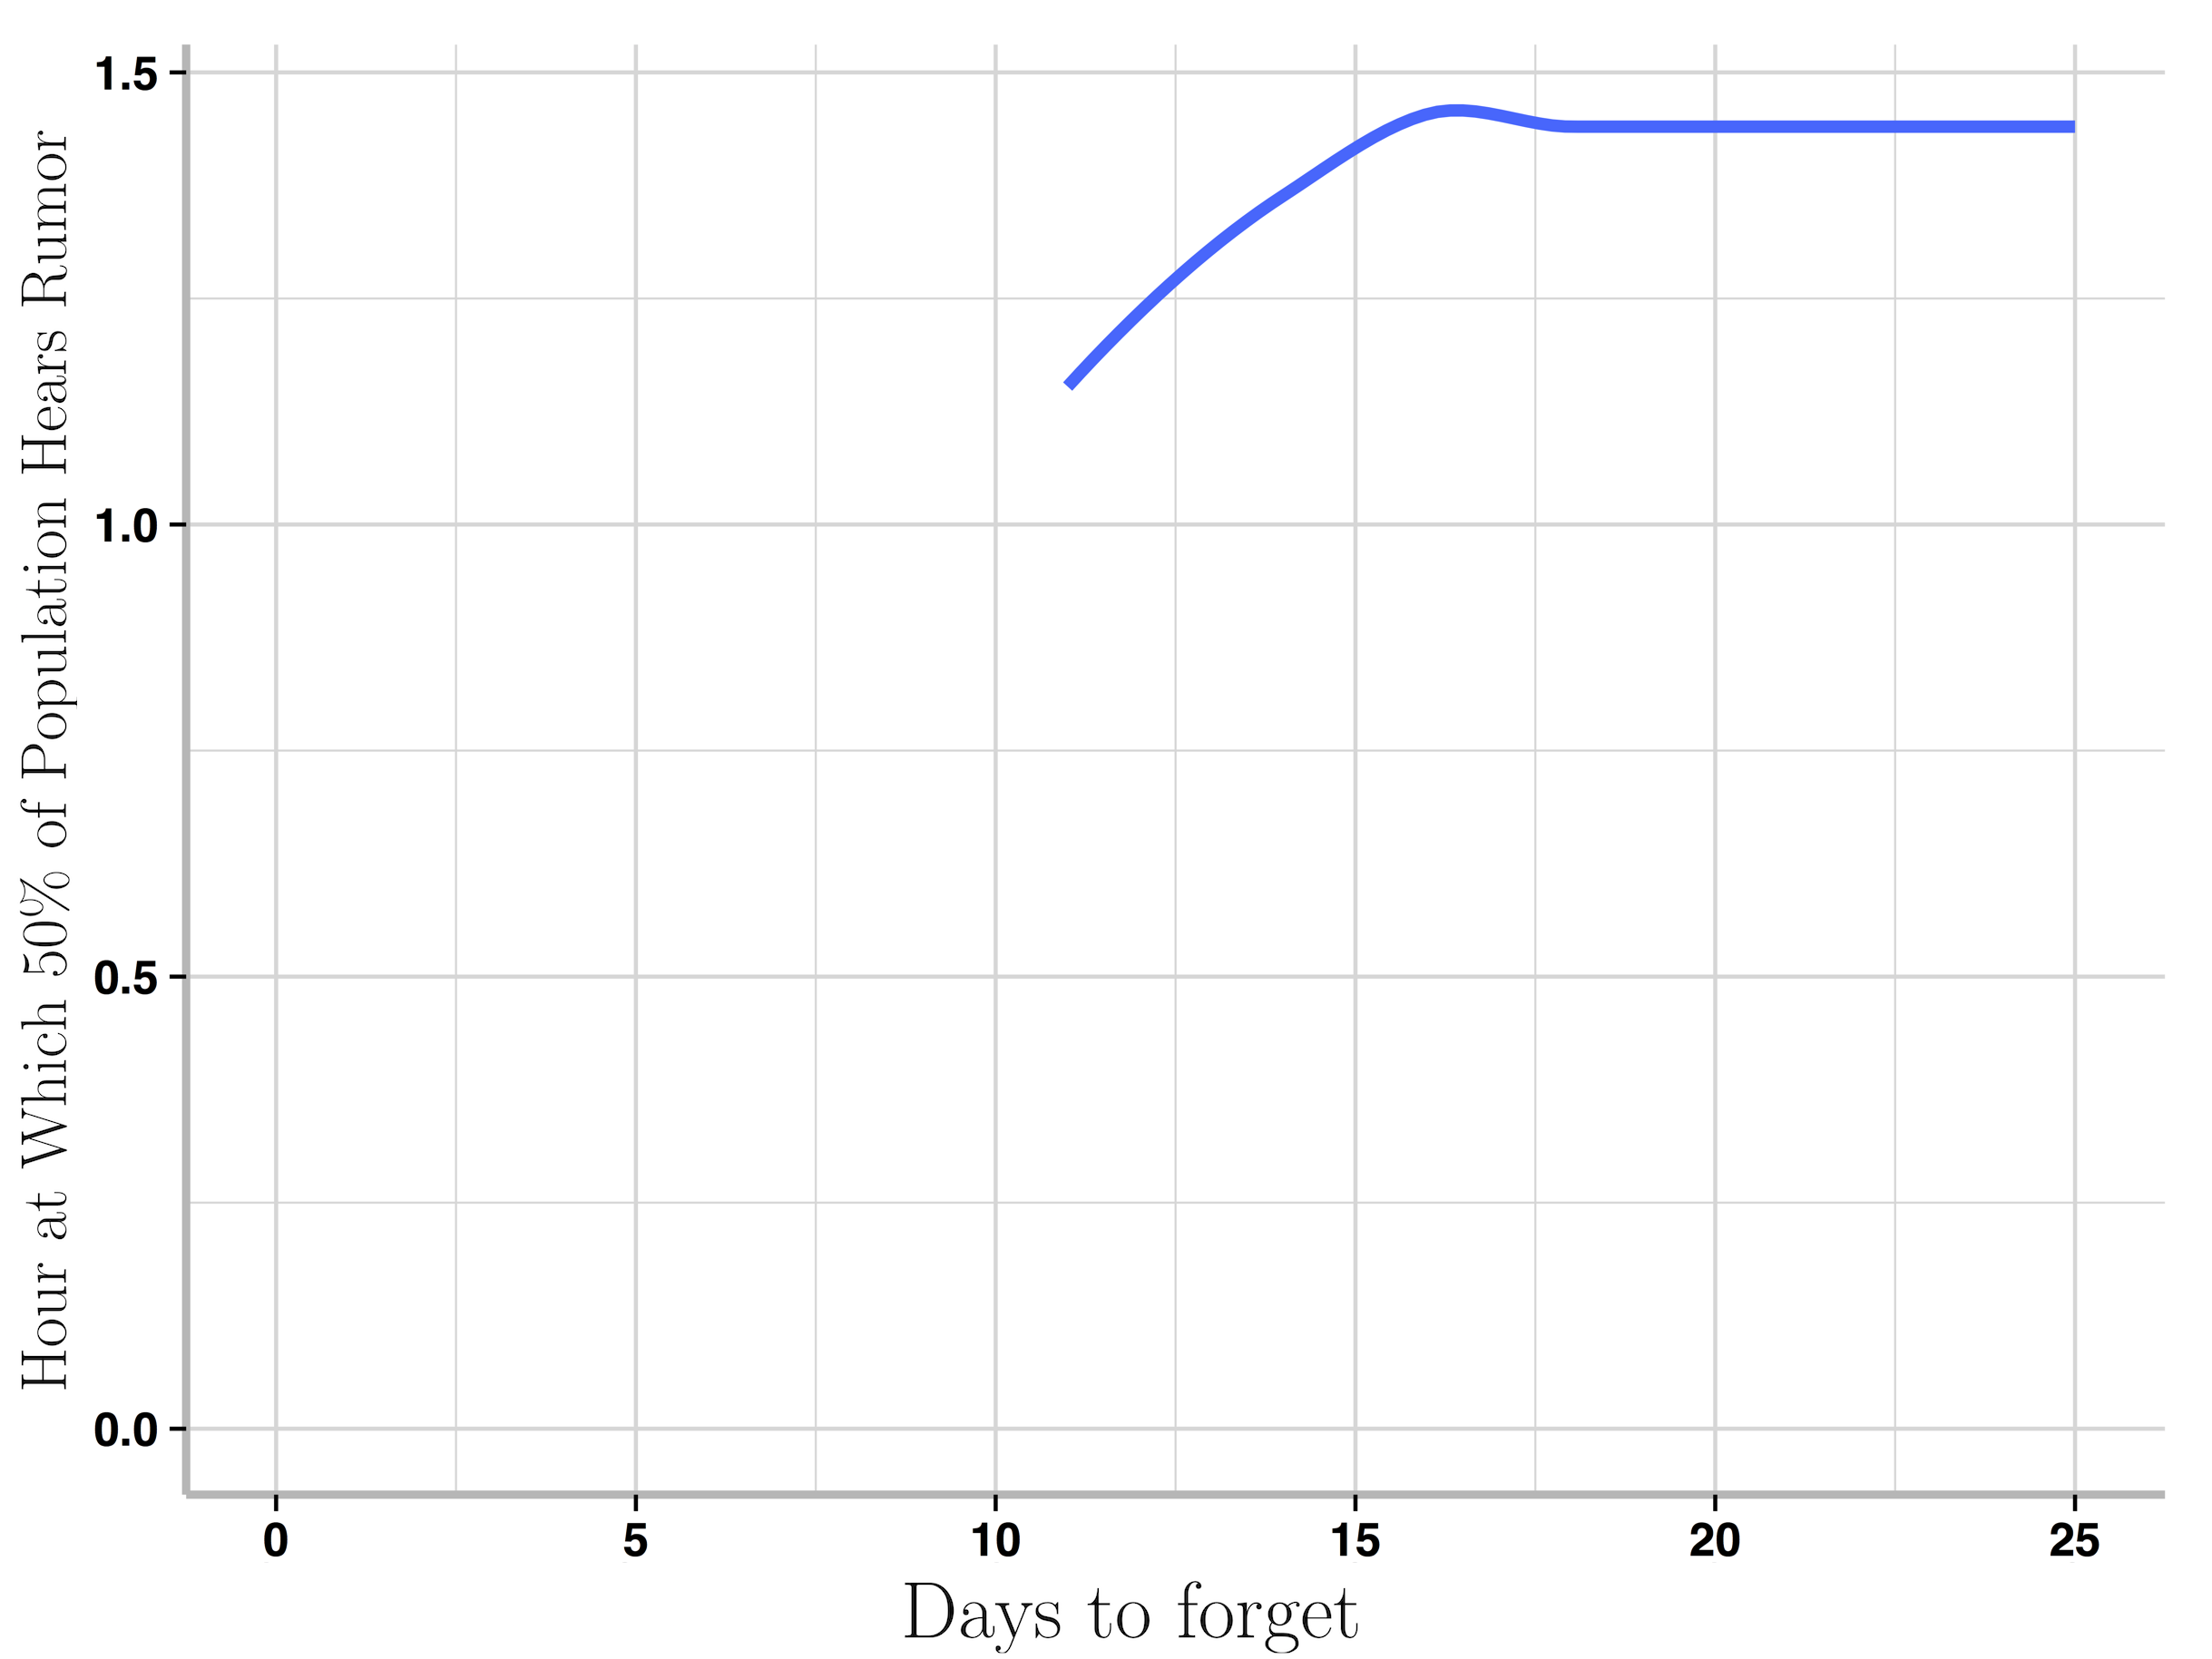
\includegraphics[width=0.7\textwidth]{figures/figure4}
  \caption{Results of the sensitivity analysis of parameter $ d $ (average days to forget) in the differential model.
The hour that 50\% of the population heard the rumor is recorded for each value of $ d $.}
\label{fig:figure4}
\end{figure}

Looking at Figures~\ref{fig:figure2},~\ref{fig:figure3}, and~\ref{fig:figure4}, increases in credibility decrease the amount of time until the rumor spreads to the majority of the population.
The increase in average days to forget increases the time by which half of the population has been exposed to the rumor.
The sensitivity analysis indicated that the time to reach the steady state depends most heavily on the $\alpha$ values.
As $ \alpha $ increases, the time at which 75 percent of the population hear the rumor increases.
When varying parameters, the $ \alpha_2 $ value was a constant double of the $ \alpha_1 $ value.

\begin{figure}[H]
\captionsetup{width=0.8\textwidth}
\centering
    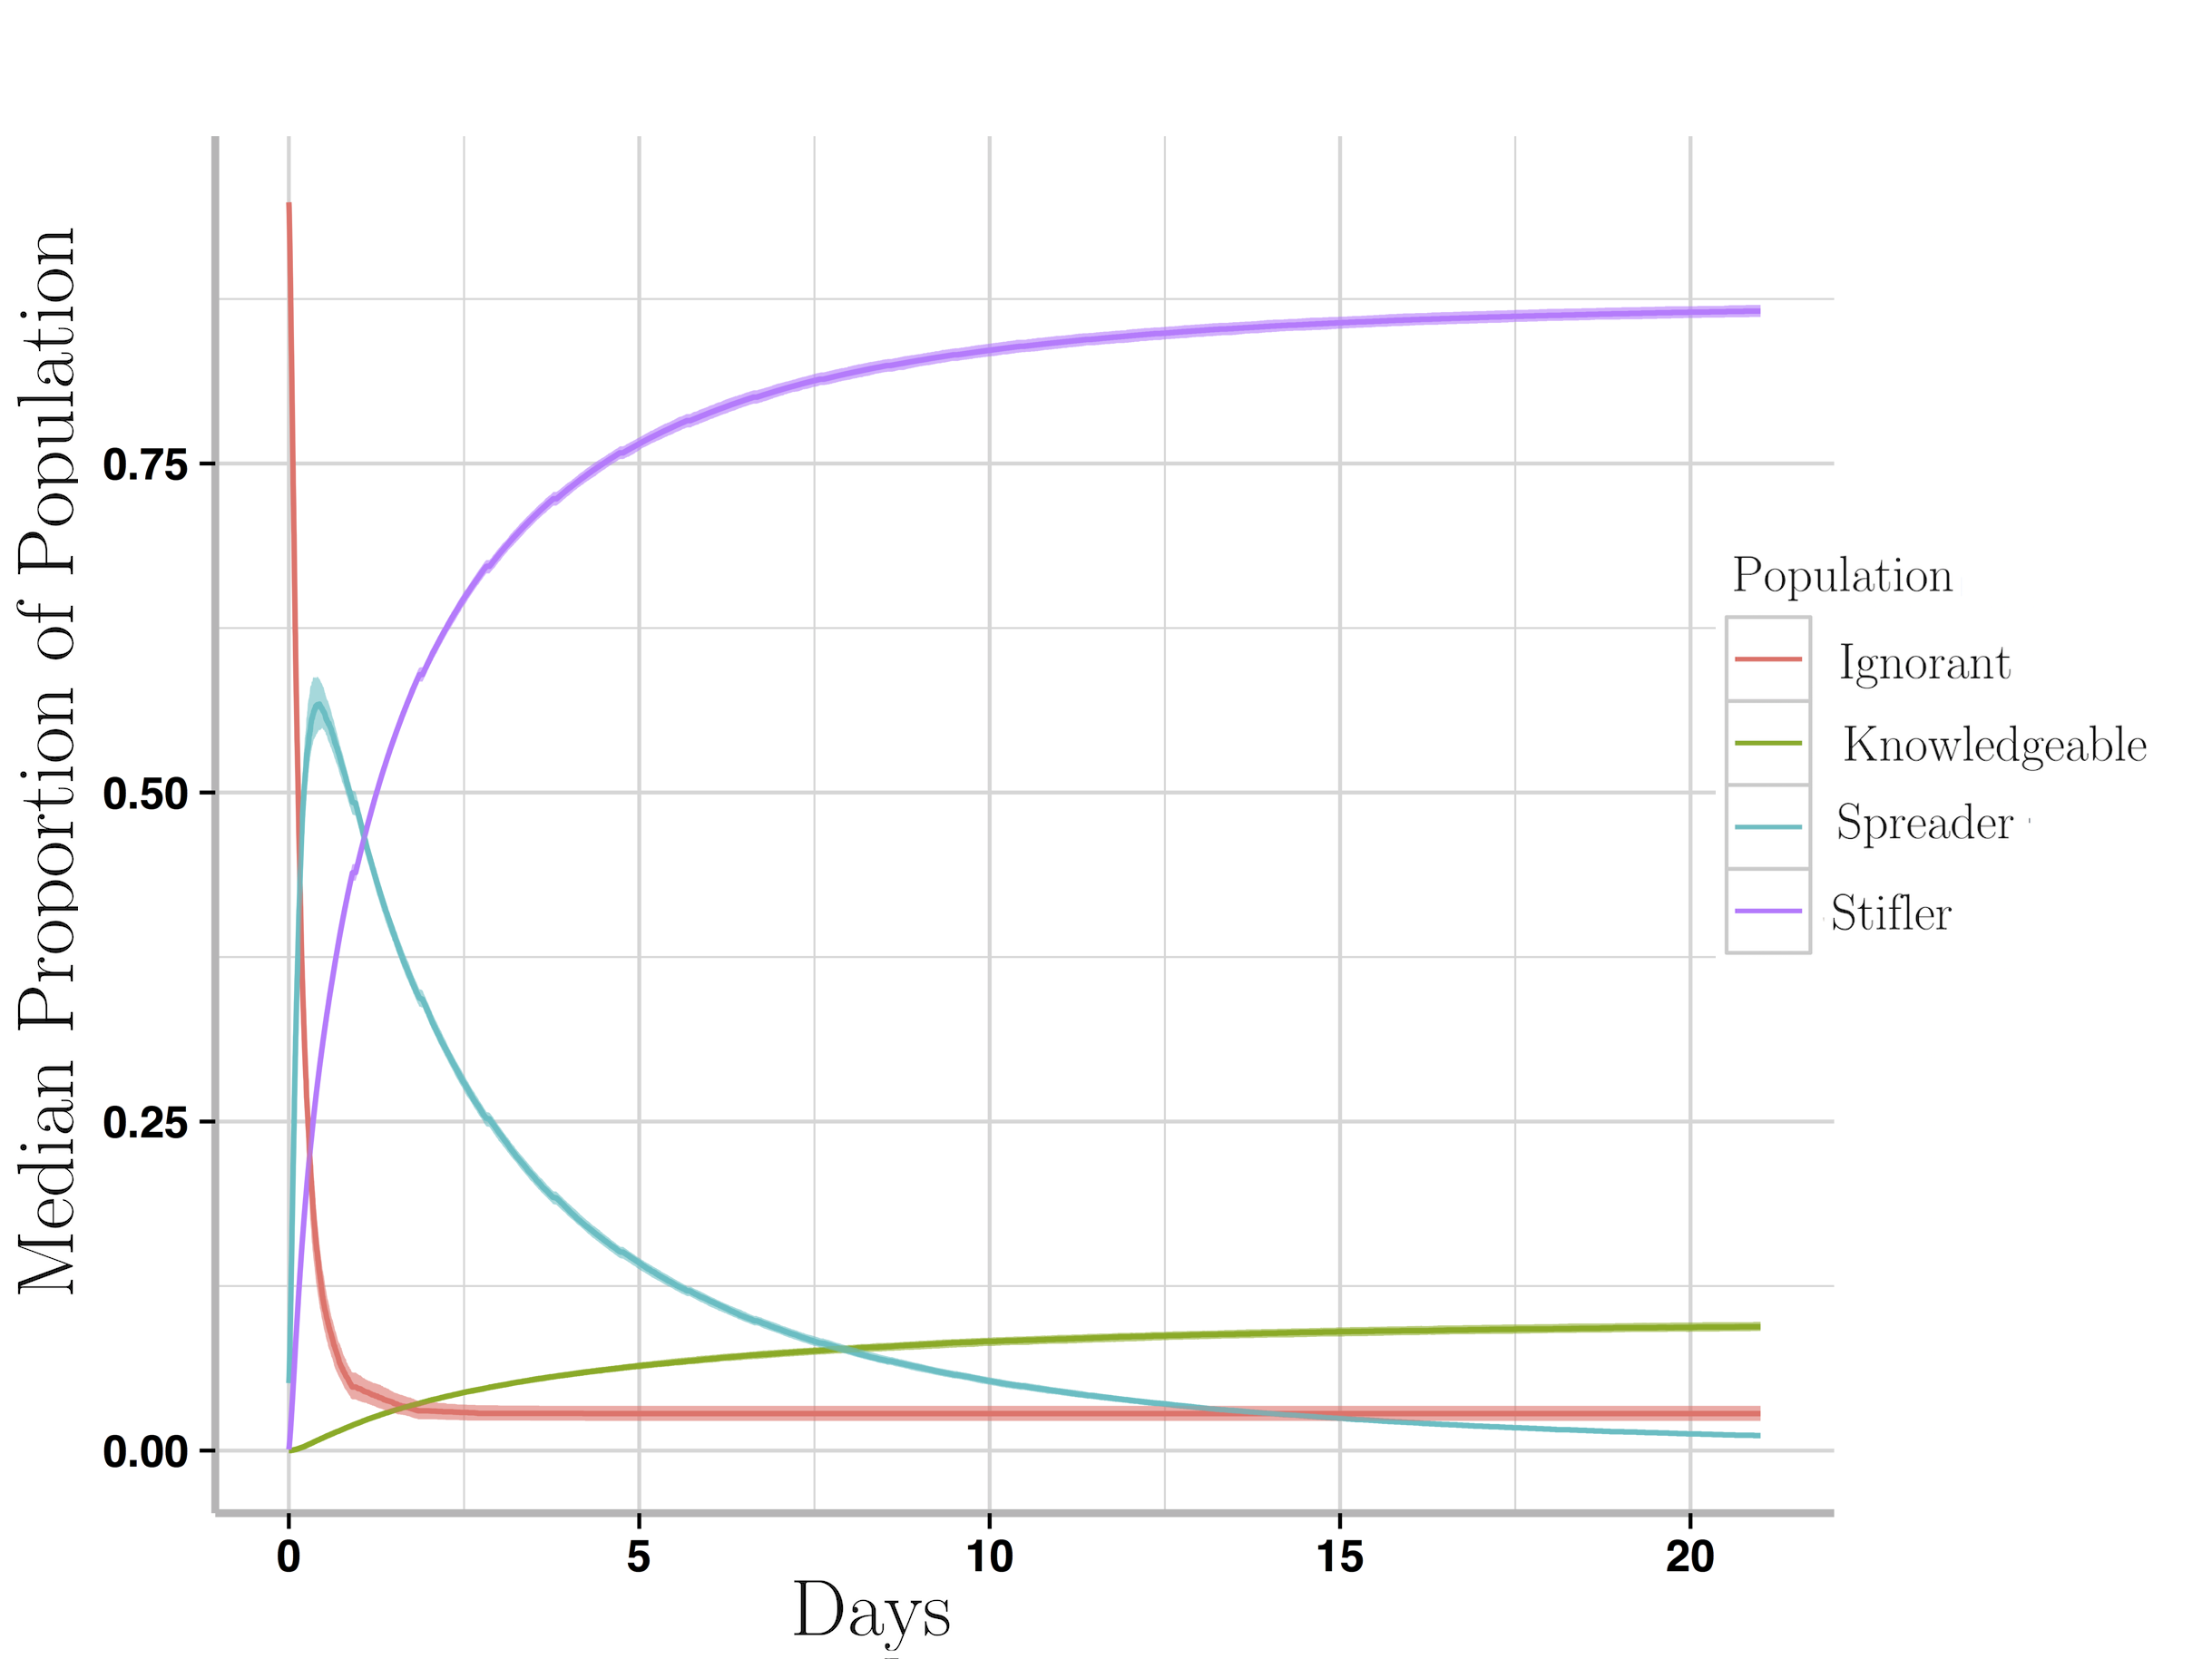
\includegraphics[width=0.7\textwidth]{figures/figure5}
  \caption{Results of the agent-based model.
Solid line indicates median proportion of population across the 400 trials; shadow indicates IQR.}
\label{fig:figure5}
\end{figure}

By comparison, in the analogous agent-based model (Figure~\ref{fig:figure5}) there are some individuals who do not hear the rumor at all by the end of the simulation.

\begin{figure}[H]
\captionsetup{width=0.8\textwidth}
\centering
    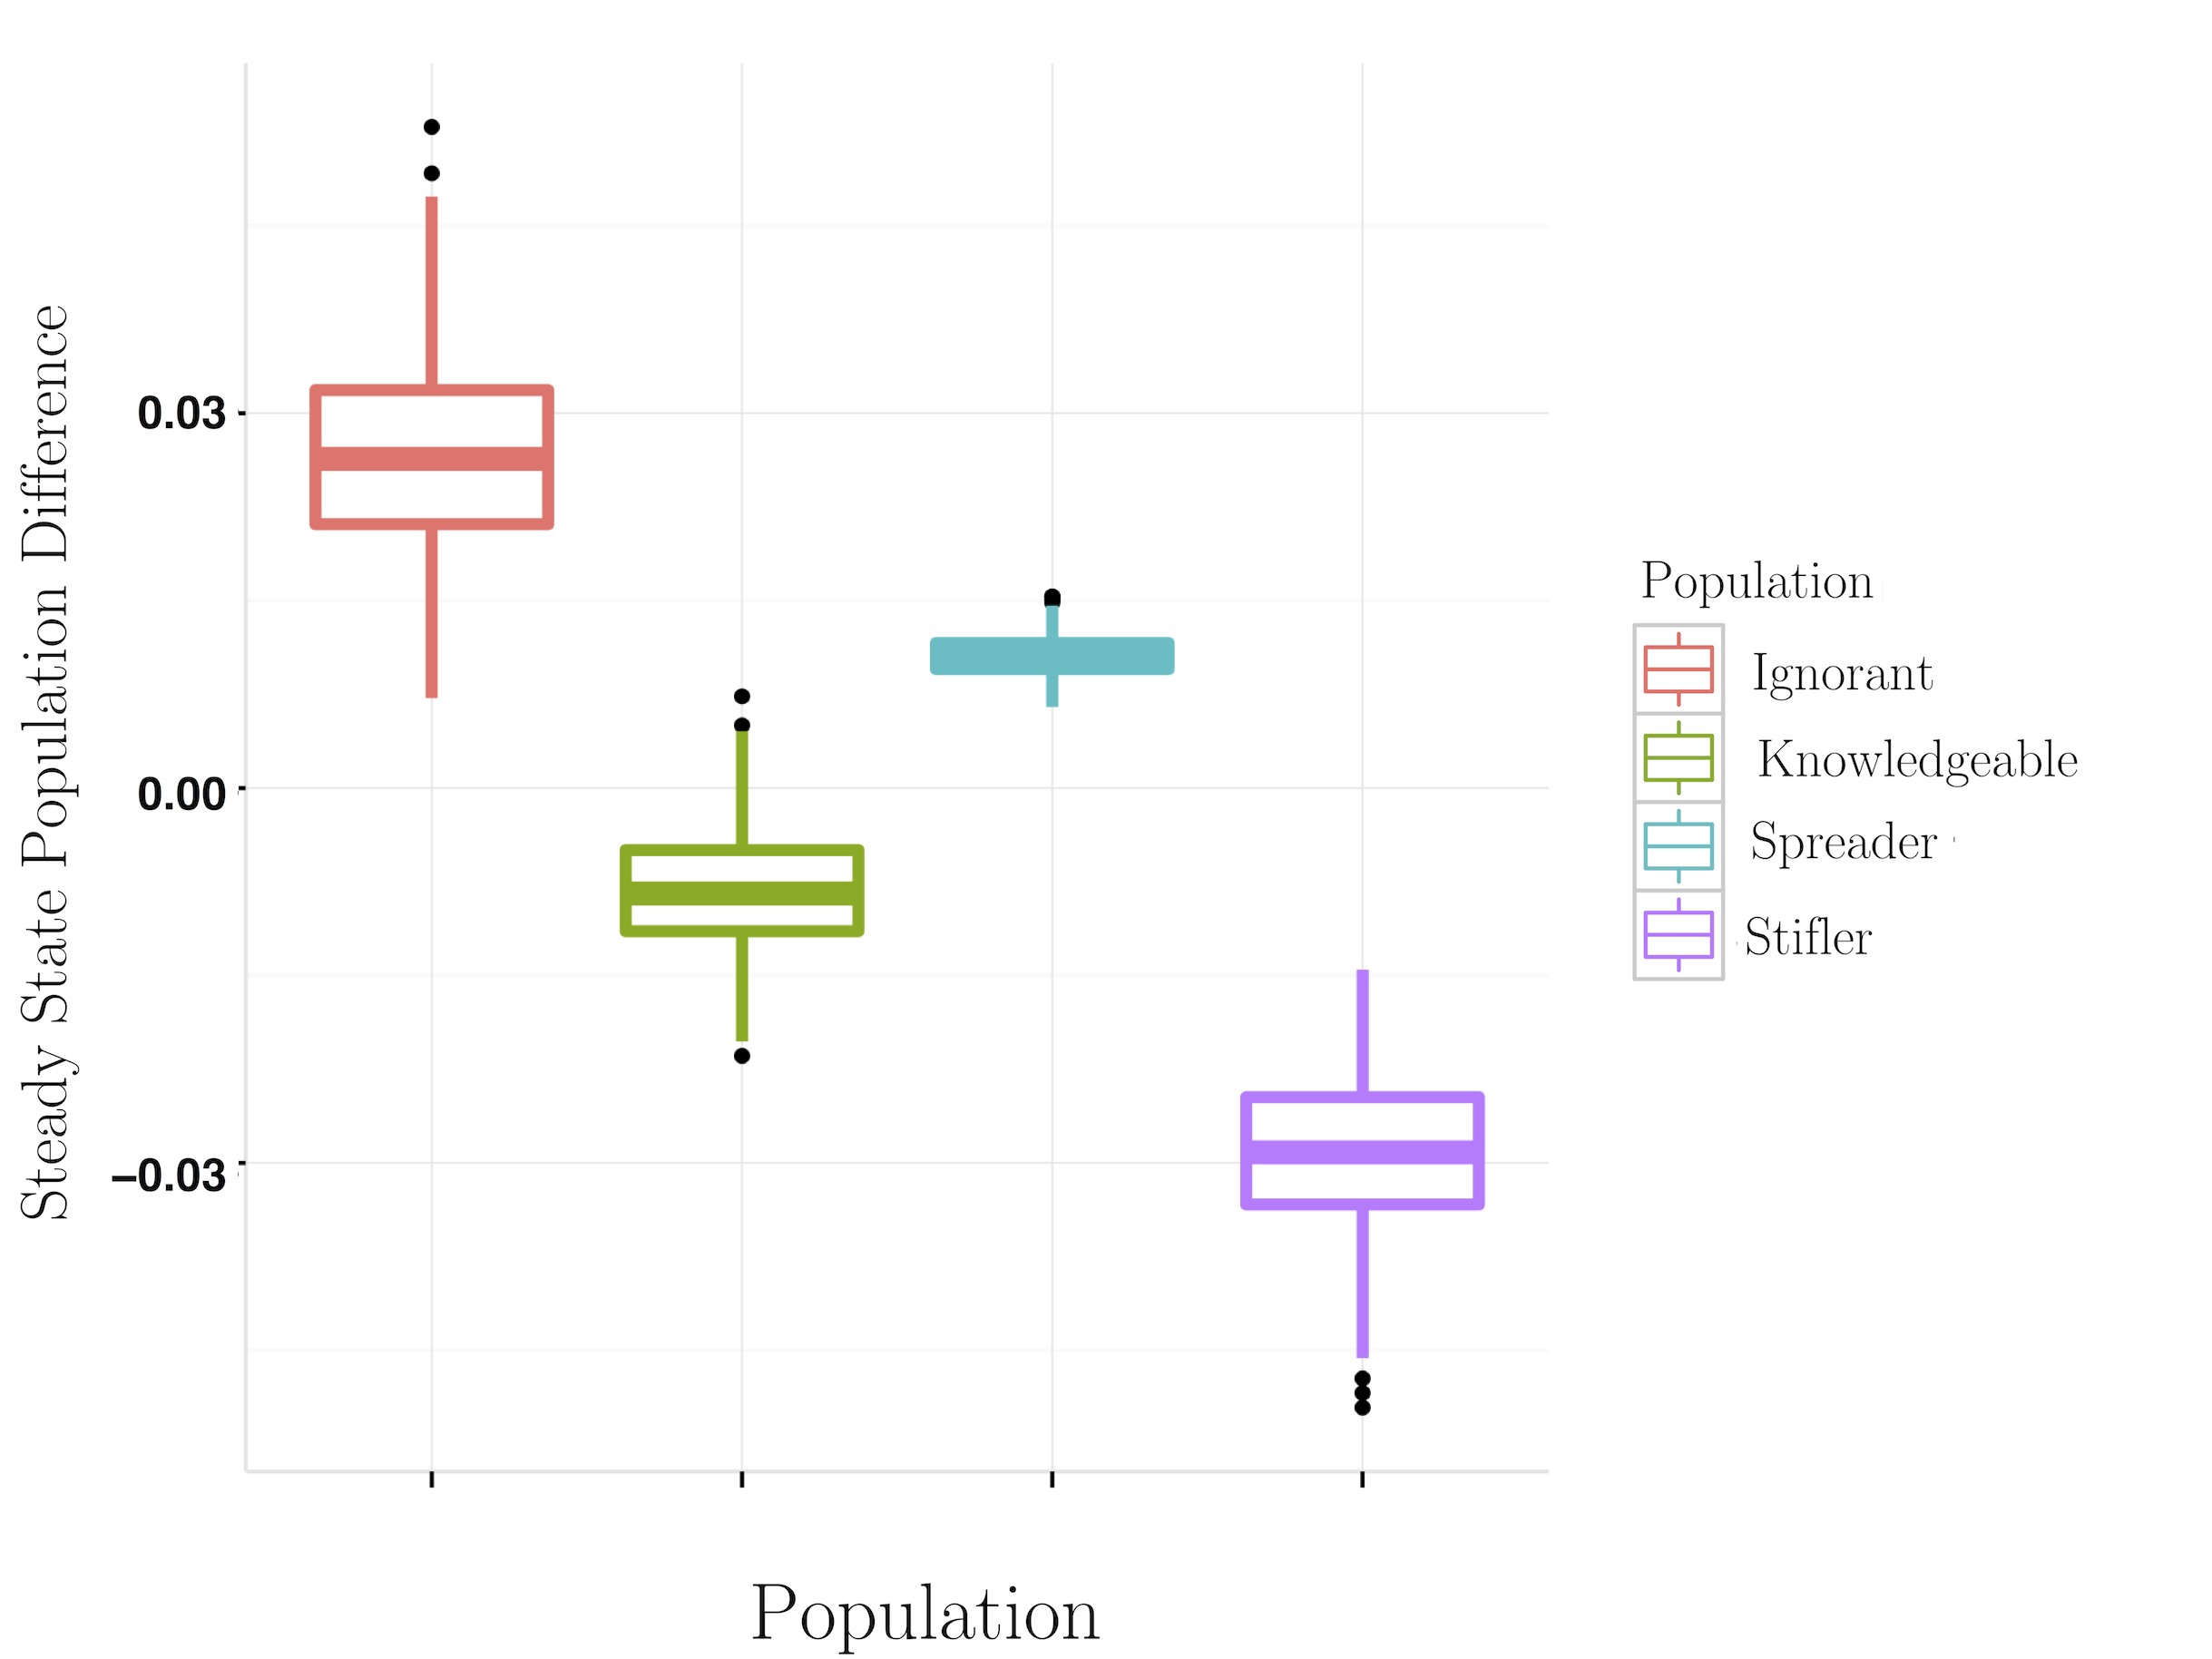
\includegraphics[width=0.7\textwidth]{figures/figure6}
  \caption{Box-and-whisker plot comparing the steady states in Figure~\ref{fig:figure1} (differential model) and the end states in Figure~\ref{fig:figure5} (Agent-based model).}
\label{fig:figure6}
\end{figure}

In this agent-based model, as expected in a stochastic model, there are pockets of ``ignorance'' that remain.
Additionally, the slope of the population graphs are more gradual, rather than moving sharply, as in the differential model.
While the dynamics of how the differential model and the simple agent-based model reached their steady-states is different, the end states are generally similar, as seen in Figure~\ref{fig:figure6}.
This shows a direct comparison of the steady states from the differential model shown in Figure~\ref{fig:figure1} and the stochastic end states from the agent-based model in Figure~\ref{fig:figure5} Though the differential model has no network, and is deterministic, we find that the agent-based model ends with essentially the same steady states.
Both models seem to confirm that with the baseline $\alpha$ values we chose, most people end up as rumor stiflers and, most people will be exposed to the rumor.
Very few people end up forgetting the rumor entirely.

\subsection{Feature-Vector, Agent-Based Model}
\label{subsec:featvect}

\begin{figure}[H]
\captionsetup{width=0.8\textwidth}
\centering
    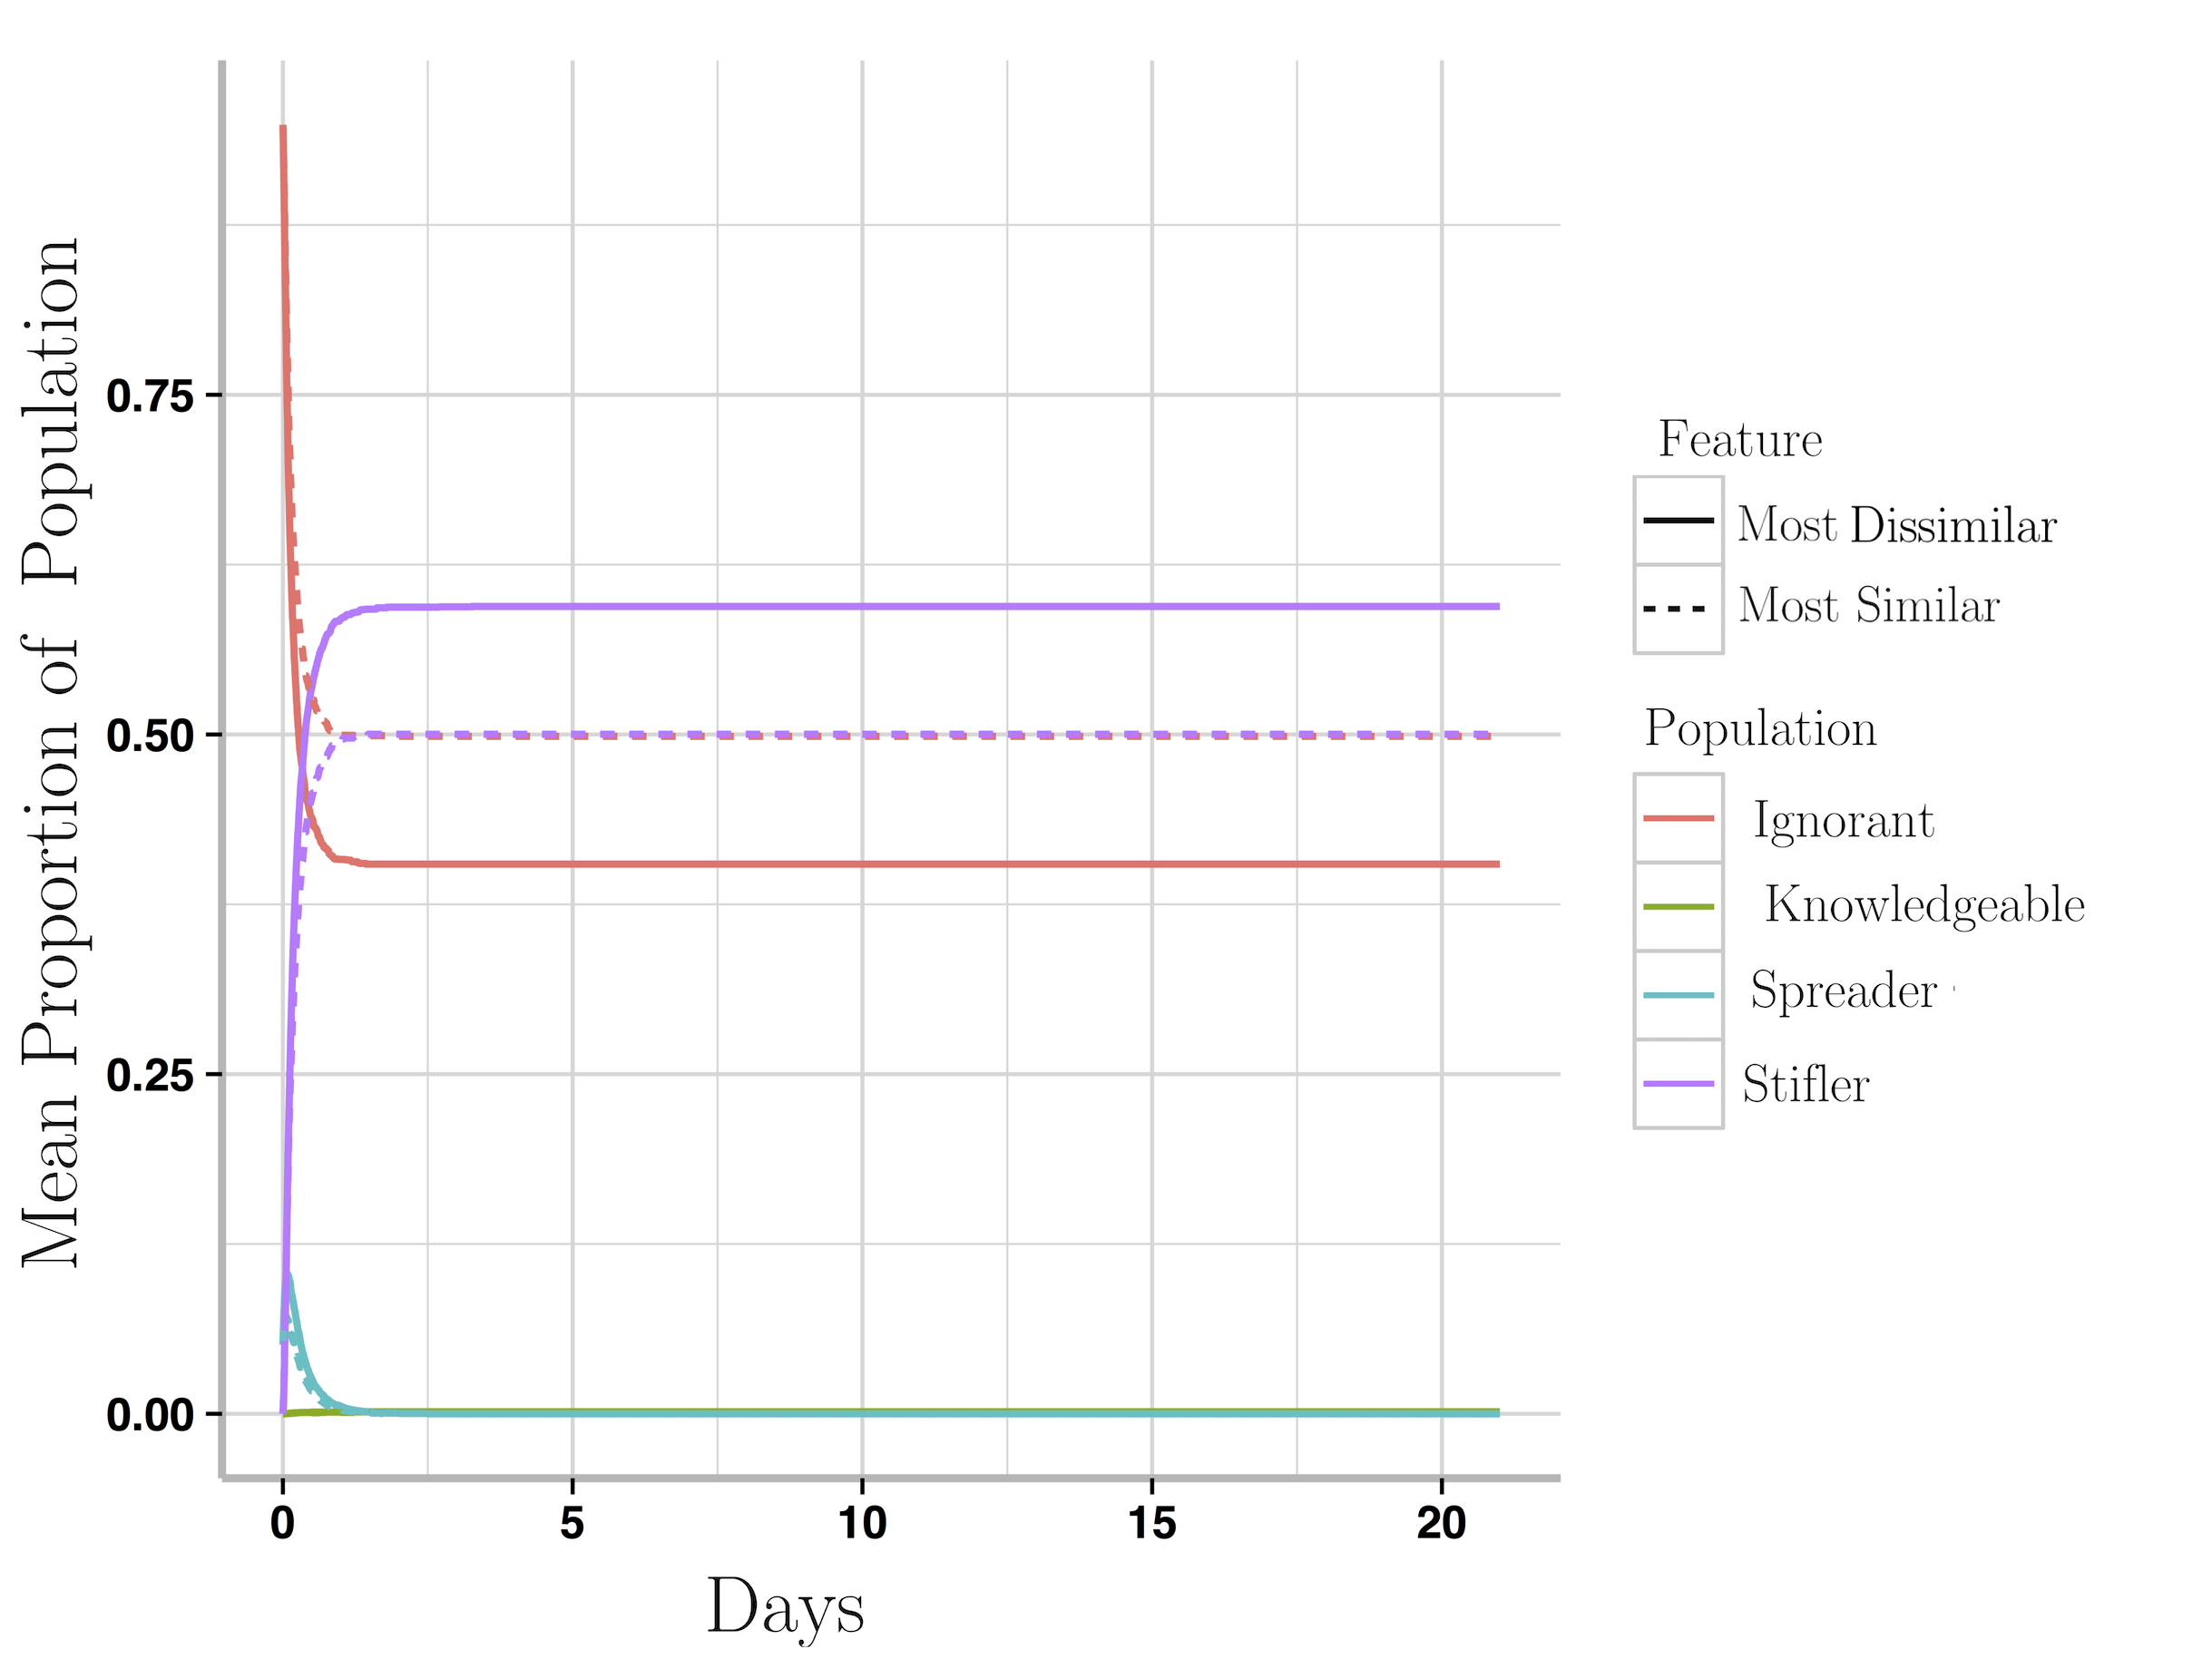
\includegraphics[width=1\textwidth]{figures/figure7}
  \caption{ Results of the most and least similar feature vectors to the population in the agent-based model (average across $ 300 $ trials).}
\label{fig:figure7}
\end{figure}

\begin{figure}[H]
\captionsetup{width=0.8\textwidth}
\centering
    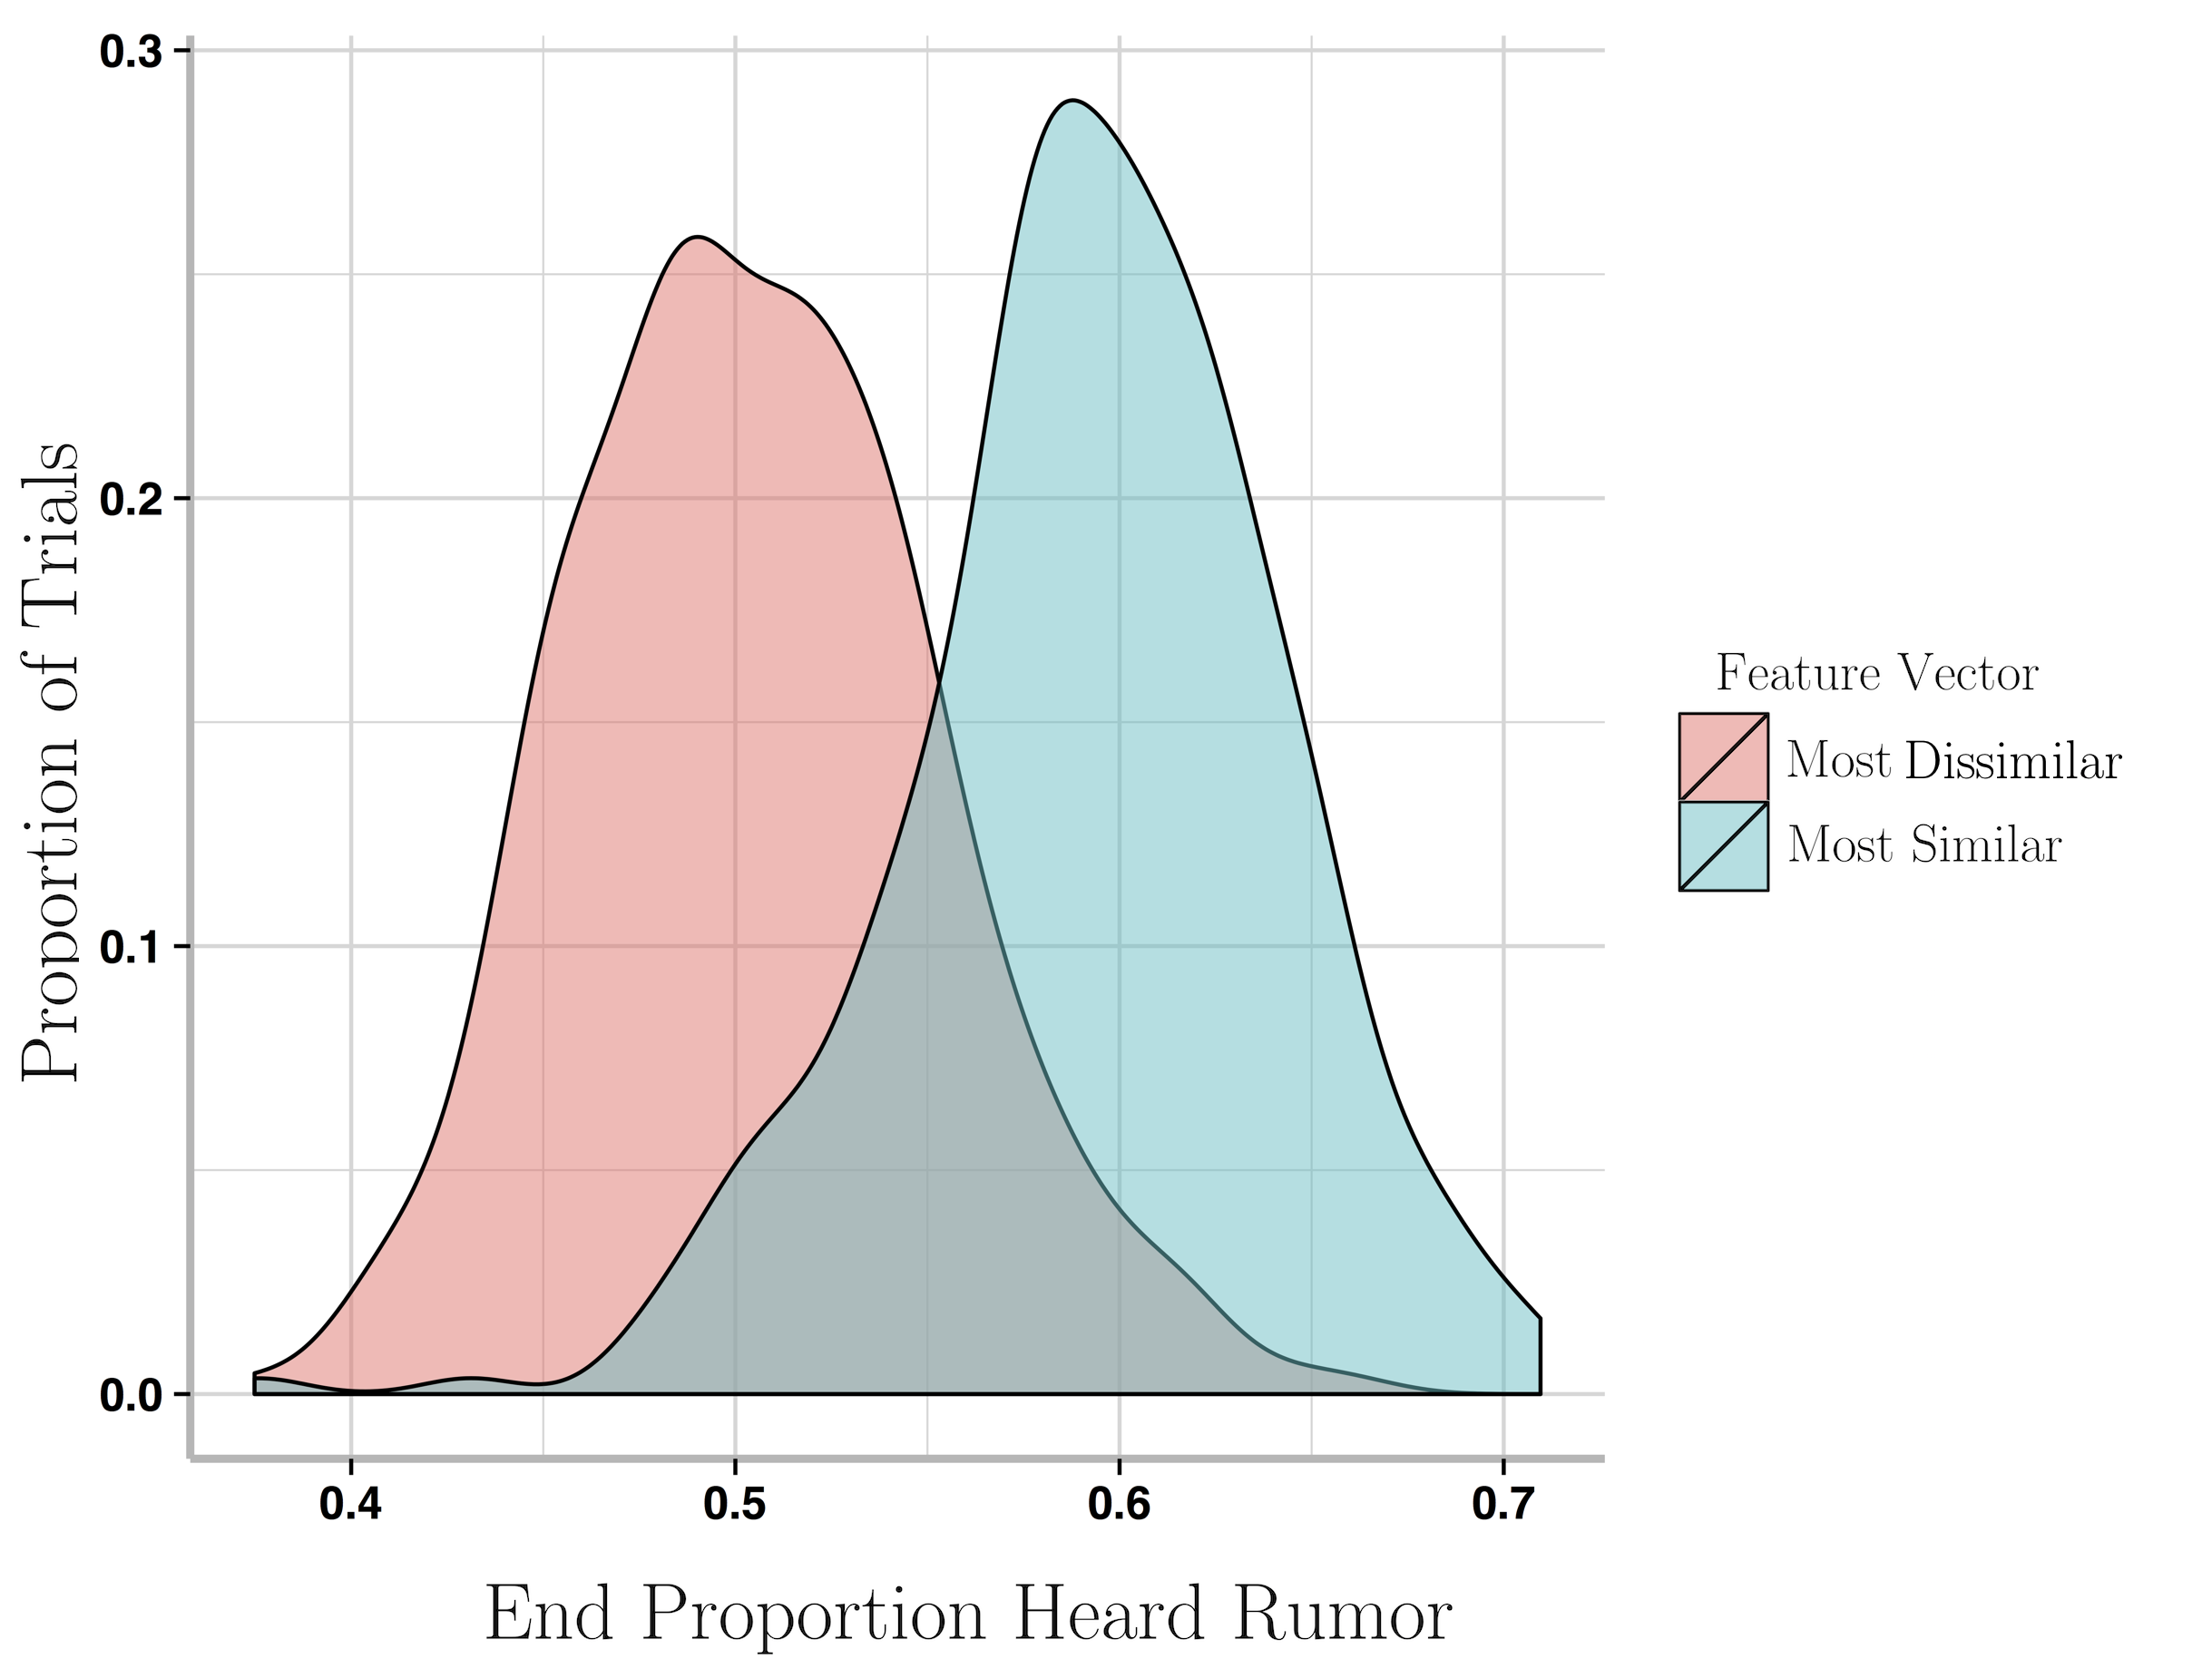
\includegraphics[width=0.7\textwidth]{figures/figure8}
  \caption{ Density of the proportion of the population who heard the rumor after $ 22 $ days with the most and least similar rumors ($ 300 $ trials).}
\label{fig:figure8}
\end{figure}

\begin{figure}[H]
\captionsetup{width=0.8\textwidth}
\centering
    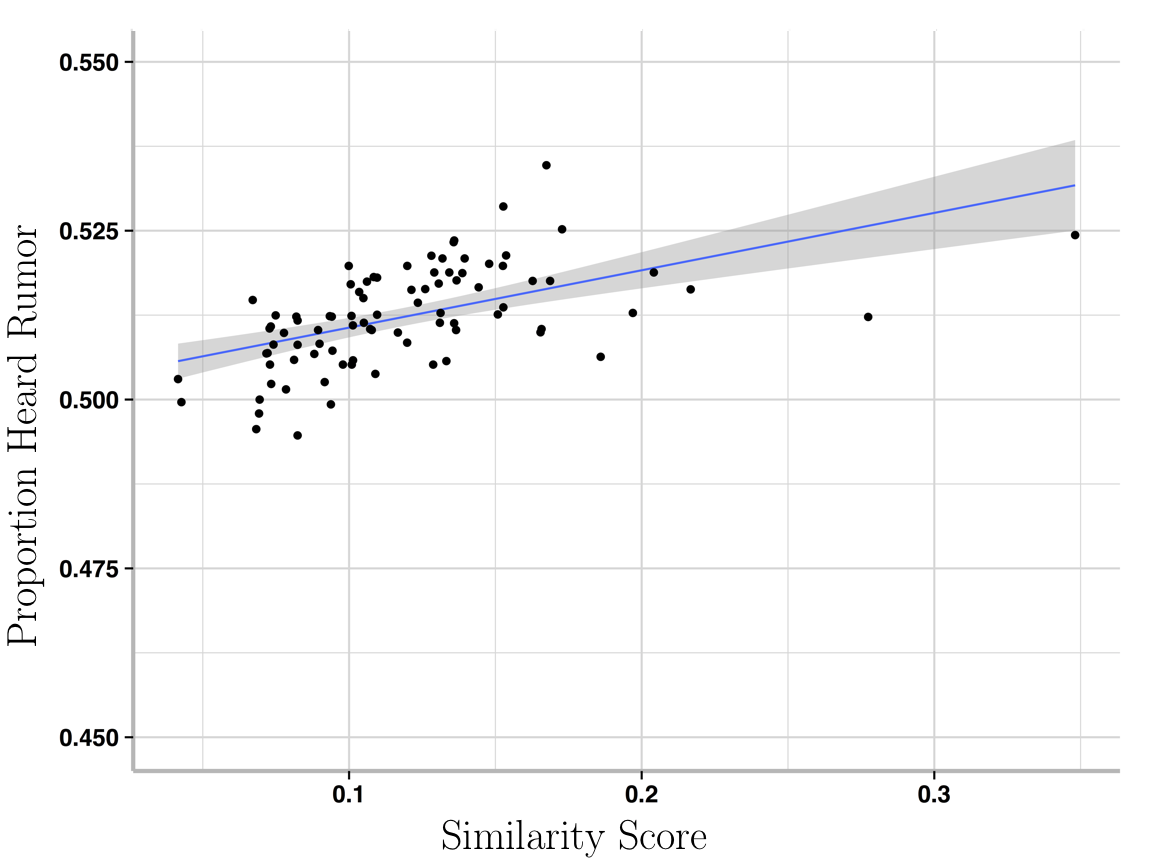
\includegraphics[width=0.7\textwidth]{figures/figure9}
  \caption{ Linear model of the relationship between the final percentage of the population heard rumor and average similarity score of the feature vector ($ r~=~0.538 $).
Shading designates the 95\% confidence interval.}
\label{fig:figure9}
\end{figure}

When the similarity score is added, even the most similar rumor dies out, as seen in Figure~\ref{fig:figure7}.
This plot is identical to Figure~\ref{fig:figure1} and Figure~\ref{fig:figure5}, but is the stochastic agent-based case.
However, the average similarity score of a rumor with the population does affect the spread (Figure~\ref{fig:figure8}).
The most similar rumor to the population spreads to more of the population than does the least similar.
The trend from the other feature vectors supports this claim, as demonstrated by Figure~\ref{fig:figure9}.
The predictive power of the similarity in predicting the number of individuals who heard the rumor is decent where the bulk of the data lies.
(n.b.\ the way that we generated most and least similar feature vectors did not guarantee that they were the absolute most or least similar to the population.
To make the most similar vector, we rounded the total proportion of each feature in the entire population to either $ 1 $ or $ 0 $ to make it binary.
The least similar vector is the logical complement of the most similar one.
Therefore, in randomly generating feature vectors, we ended up with a few that were less similar than the ``least similar'' feature vector.)
